\section{THE $m_{max}-M_{ecl}$ RELATION}
The $m_{max}-M_{ecl}$ relation, as shown in Fig.\ref{fig:max-mecl}has been analytically presented in Weidner  Kroupa (2004), observationally
established by Weidner  Kroupa (2006) and refined in Weidner et al. (2010), while already briefly theoretically discussed
in Reddish (1978).\\
It signifies that the typical upper mass limit to which the IMF is sampled, m max , changes systematically
with the stellar mass of the cluster, $M_{ecl}$ .
\begin{figure}[h]\centering
	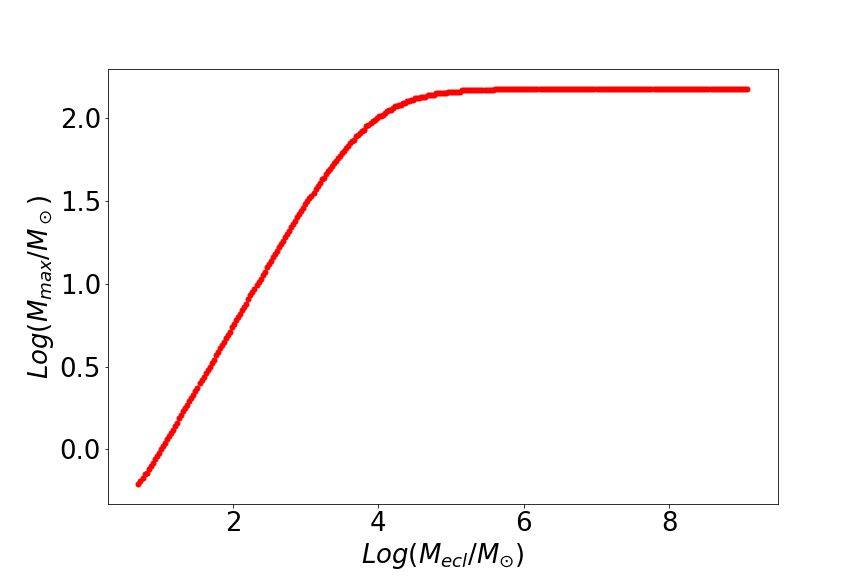
\includegraphics[width=0.7\linewidth]{max-melc.png}
	\caption{The mass of the most-massive star $(m_{max})$ in an embedded cluster versus the stellar mass of the young dynamically
		un-evolved ”embedded” cluster $(M_{ecl})$.The solid lines through the data points are the analytical $m_{max}-M_{ecl}$
		relation when using a fundamental upper mass limit, $m_{max,*}$ , of $150 M_{\odot}$.}
	\label{fig:max-mecl}
\end{figure}
For the clusters for which the number of stars above a mass limit or within a mass range are given in the literature,
the cluster mass,  $M_{ecl}$  , is calculated by assuming a canonical IMF from $0.01$ to $150 M_{\odot}$ and extrapolating
to the total population from the observational mass limits.
\subsection{The maximum stellar mass and cluster formation}
Assuming the stellar IMF is a continuous density distribution function and that
clusters are filled with stars distributed according to the stellar IMF, this can
be generalized by stating that each cluster can have only one most massive star,
\begin{equation}
1=\int_{m_{max}}^{m_{max*}}\xi(m')dm',
\end{equation}
with,
\begin{equation}
M_{}ecl}(m_{max})=\int_{m_{low}}^{m_{max}} m' \xi(m')dm',
\end{equation}
as a further condition, as above. These two equations need to be solved numeri-
cally and give the semi-analytical relation $ m_{max}= \eta (M_{ecl} )$(Weidner & Kroupa
2004). It is plotted in fig.\ref{fig:max-mecl}.
A compilation of clusters from the literature for which the cluster mass and
the initial mass of the heaviest star can be estimated (Weidner & Kroupa 2006)
shows that the cluster mass indeed appears to have a limiting influence on the
stellar mass within it. The observational data are plotted in Fig. \ref{fig:ko-re}, finding
rather excellent agreement with the semi-analytical description above.
\begin{figure}[h]\centering
	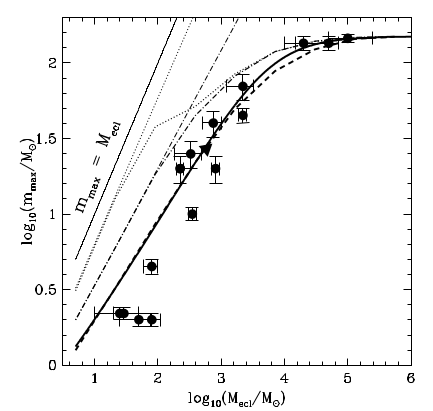
\includegraphics[width=0.7\linewidth]{ko-rev.png}
	\caption{The thick solid line shows the dependence of the mass of the most-
		massive star in a cluster on the cluster mass according to the semi-analytical	model. The thick dashed line shows the mean maximum stellar mass for sorted
		sampling. The dot-dashed lines are mass-constrained random-sampling results	with a physical upper mass limit of $m_{max*}=150M_{\odot}$ (thick line) and $10^6 M_{\odot}$(thin line). Pure random sampling models are plotted as dotted lines. The
		thick one is sampled to $m_{max*}=150M_{\odot}$ while the thin one up to $10^6 M_{\odot}$.
		The thin solid line shows the identity relation, where a “cluster” consists only of one star. The dots with error bars are observed clusters, while the triangle is a result from a star-formation simulation with an SPH code (Bonnell et al.2003). Taken from Weidner & Kroupa (2006).}
	\label{fig:ko-re}
\end{figure}


